\documentclass{anstrans}
%%%%%%%%%%%%%%%%%%%%%%%%%%%%%%%%%%%
\title{Diffusion Boundary Conditions in Flatland Geometry}
\author{Seth R.~Johnson \and Edward W.~Larsen}

\institute{Department of Nuclear Engineering \& Radiological Sciences, University of Michigan, Ann Arbor, MI, 48109}
\email{sethrj@umich.edu \and edlarsen@umich.edu}
\usepackage{amssymb}
\usepackage{microtype}
\usepackage{graphicx}
\usepackage{booktabs} % \toprule, \midrule, \bottomrule
%%% INCLUDE FILE FOR DEFINITIONS
%%% These may require various packages.

% Shortcuts in regular text
\newcommand{\degs}{\ensuremath{^\circ}}
\newcommand{\EE}[1]{\ensuremath{\times 10^{#1}}}
\newcommand{\ttimes}{\ensuremath{{}\times{}}}
\newcommand{\cclicense}{%
  \smash{\raisebox{-0.45ex}{%
  \setlength{\unitlength}{1em}%
  \begin{picture}(1,1)%
    \put(0.5,0.5){\circle{1}}
    \put(0.5,0.5){\hbox to 0pt{\hss\raisebox{-.45ex}{\tiny\textsf{CC}}\hss}}
  \end{picture}%
  }}%
  \hskip -1em%
  \href{http://creativecommons.org/licenses/by-nc-sa/3.0/}%
  {\ \hskip 1em \textsf{BY-NC-SA}}%
}

%\newcommand{\horizsep}{{\par\noindent\centering\rule[.25ex]{.75\columnwidth}{2pt}\par}}
\newcommand{\horizsep}{\vspace{\baselineskip}\noindent\hspace{\stretch{1}}$
\ast\qquad \ast\qquad \ast\qquad
$ \hspace{\stretch{1}} \vspace{\baselineskip}}
\newcommand{\pytrt}{\textsf{PyTRT}}

% Research
\newcommand{\lop}[1]{\mathcal{L}\!\left[#1\right]}
\newcommand{\lopinv}[2]{\mathcal{I}_{#1}\!\left[#2\right]}
\newcommand{\Dtens}{\mat{D}}
\newcommand{\Etens}{\mat{E}}
\newcommand{\Identitytens}{\mat{I}}
\newcommand{\APone}{AP$_1$}
\newcommand{\Pone}{P$_1$}
\newcommand{\SN}{S$_N$}%{S$_\text{N}$}%{$S_N$}%
\newcommand{\PN}{P$_N$}%{P$_\text{N}$}%{$P_N$}%
\newcommand{\CN}{Crank--Nicolson} %Yes, it's Nic not Nich
\newcommand{\Eddington}{\mathcal{E}} %whatever symbol I decided for Eddington
\newcommand{\RadEn}{E} %whatever symbol I decide for radiation energy
\newcommand{\Sigmatr}{\Sigma_{\mathit{tr}}}

% Program names
\newcommand{\cpp}{\textsf{C\raisebox{0.2ex}{++}}}

% General math shortcuts
\newcommand{\ud}{\mathop{}\!\mathrm{d}}
\newcommand{\pder}[2]{\frac{\partial #1}{\partial #2}}
\newcommand{\oder}[2]{\frac{\mathrm{d} #1}{\mathrm{d} #2}}
\newcommand{\tpder}[2]{{\partial #1}/{\partial #2}} %inlined
\newcommand{\toder}[2]{{\mathrm{d} #1}/{\mathrm{d} #2}} %inlined
\newcommand{\lra}{ \quad \Longrightarrow \quad }
\newcommand{\eexp}{\mathop{}\!\mathrm{e}} % upright ``e'' for exponent
\newcommand{\expp}[1]{\exp\!\left( {#1} \right)} % exp with parentheses
\newcommand{\qeq}{\stackrel{\mathrm{?}}{=}}

% Probability
\newcommand{\expectation}[1]{\mathop{}\!\mathrm{E}\!\left[ #1 \right]}
\DeclareMathOperator{\Var}{Var} % variance

% Asymptotic analysis
\DeclareMathOperator{\Ei}{Ei} % Exponential function
\newcommand{\lapl}[1]{\mathcal{L}[{#1}]} %laplace

%change the Re and Im operators from fancy curly letters
\DeclareMathOperator{\MathOpRe}{Re}
\renewcommand{\Re}{\MathOpRe}
\DeclareMathOperator{\MathOpIm}{Im}
\renewcommand{\Im}{\MathOpIm}

%imaginary ``i'' , upright 'i' or \imath
\newcommand{\iimag}{\mathrm{i}}

% Finite differences
\newcommand{\hot}{\text{h.o.t.}}
\newcommand{\inv}{^{-1}}

% Numerical Linear Algebra
\newcommand{\conj}{^{\ast}} % complex conjugate (transpose)
\newcommand{\norm}[1]{\left\| #1 \right\|} % double pipe
\newcommand{\abs}[1]{\left| #1 \right|} % single pipe
\newcommand{\eps}{\varepsilon}
\DeclareMathOperator{\fl}{fl}

\DeclareMathOperator{\acosh}{arccosh} 

% Define a command to write a nice-looking element, e.g. 4,2 He
\newcommand{\elem}[3]{\ensuremath{{}^{{#1}}_{{#2}}\mathrm{{#3}}}}

% Vector definitions
\newcommand{\mat}[1]{\mathbf{#1}} %matrix is bold upright
\renewcommand{\vec}[1]{\bm{#1}} %vector is bold italic
\newcommand{\op}[1]{\mathsf{#1}} % ``operator'' is sans serif

\newcommand{\vd}{\bm{\cdot}} % slightly bold vector dot
\newcommand{\del}{\vec{\nabla}} % gradient (Del) is bold
\newcommand{\grad}{\vec{\nabla}} % gradient

%\newcommand{\abr}[1]{\langle {#1} \rangle}
\newcommand{\abr}[1]{\left\langle {#1} \right\rangle} % angle brackets for avg.

%% topbox is useful in extended definitions of math terms inside an align
\newcommand{\topbox}[2][0.6]{\parbox[t]{#1\columnwidth}{\raggedright{}#2}}

% commands to make text in math mode appear as zero-width (better-looking
% integrals/sums, e.g.)
% from mathmode.pdf page 74, or Alexander R. Perlis ``A complement to \smash,
% \llap, and \rlap''

\def\mathllap{\mathpalette\mathllapinternal}
	\def\mathllapinternal#1#2{%
	\llap{$\mathsurround=0pt#1{#2}$}%
}
\def\clap#1{\hbox to 0pt{\hss#1\hss}}%
\def\mathclap{\mathpalette\mathclapinternal}%
\def\mathclapinternal#1#2{%
	\clap{$\mathsurround=0pt#1{#2}$}%
}
\def\mathrlap{\mathpalette\mathrlapinternal}%
\def\mathrlapinternal#1#2{%
	\rlap{$\mathsurround=0pt#1{#2}$}%
}


% graphics paths
\graphicspath{{/Users/seth/_research/figures/}}
\makeatletter
\def\input@path{{/Users/seth/_research/figures/}}
\makeatother

\renewcommand{\bottomfraction}{0.99}
\renewcommand{\topfraction}{0.99}
\setlength{\parskip}{0pt}

%\usepackage{setspace}
%\doublespacing

\date{2011/05/30}
%%%%%%%%%%%%%%%%%%%%%%%%%%%%%%%%%%%
\begin{document}
%%%%%%%%%%%%%%%%%%%%%%%%%%%%%%%%%%%%%%%%%%%%%%%%%%%%%%%%%%%%%%%%%%%%%%%%%%%%%%%%
\section{Introduction}
``Flatland'' is a fictional two-dimensional universe in which particles are
constrained to exist and
travel in a 2-D plane \cite{Asa2008}. Because the flatland phase space is
$(x,y,\omega)$ with \emph{one} angular variable (the azimuthal~$\omega$),
rather than the
standard 2-D $(x,y,\mu,\omega)$ with \emph{two} angular variables (the
polar cosine~$\mu$ and the azimuthal~$\omega$),
flatland is a computationally simpler testing ground that retains the
complexity of multidimensional geometry. For this reason, flatland has recently
been used in the development and testing of multi-D transport methods
\cite{Lar2009c,Joh2011,Tra2011}.

Previous work has shown that the 3-D diffusion coefficient
$\frac{1}{3\sigma}$ differs from the flatland diffusion coefficient
$\frac{1}{2\sigma}$, but accurate boundary conditions for the flatland
diffusion equations have not been derived. An accurate diffusion
boundary condition is needed for benchmarking new transport methods against
diffusion solutions. Thus, in the following we \textsl{(i)} derive ``Marshak''
and ``variational'' boundary conditions for the flatland diffusion equation,
and \textsl{(ii)} demonstrate their accuracy via numerical
simulations.

%%%%%%%%%%%%%%%%%%%%%%%%%%%%%%%%%%%%%%%%%%%%%%%%%%%%%%%%%%%%%%%%%%%%%%%%%%%%%%%%
\section{Analysis}
The steady-state, monoenergetic transport equation is
\begin{equation}\label{eq:generalTransport}
  \vec{\Omega}\vd \grad \psi + \sigma \psi
  = \frac{c \sigma}{\gamma_0} \int_{\Omega} \psi \ud\Omega + \frac{q}{\gamma_0}
  \quad \vec{x}\in V,\ \vec{\Omega}\in \Omega \,,
\end{equation}
where the direction vector $\vec{\Omega}$, the unit ``sphere'' $\Omega$, and
the constant $\gamma_0$ depend on whether the geometry
is flatland or 2-D. We consider a specified incident boundary condition:
\begin{equation} \label{eq:ssBndy}
  \psi(\vec{x}, \vec{\Omega}) = \psi^b(\vec{x}, \vec{\Omega})\,,
  \quad \vec{x}\in \partial V,\ \vec{\Omega} \vd \vec{n} < 0\,.
\end{equation}

In 2-D geometry, $\vec{\Omega}=\sqrt{1-\mu^2} \cos \omega \vec{i} +
\sqrt{1-\mu^2} \sin \omega \vec{j}$; and in flatland, $\vec{\Omega}=\cos \omega
\vec{i} + \sin \omega \vec{j}$. The domain of angular integration $\Omega$ in
2-D is $-1\le\mu\le1$, $0 \le \omega < 2\pi$; in flatland, it is $0 \le \omega
< 2\pi$. These lead to the different angular moments
\begin{equation}\label{eq:omegaIdentities}
  \gamma_m = \int_{\Omega} \abs{\vec{\Omega}\vd \vec{i}}^m \ud\Omega\,.
\end{equation}
In 2-D, $\gamma_0=4\pi$, $\gamma_1=2\pi$, and $\gamma_2=\frac{4\pi}{3}$.
In flatland, $\gamma_0=2\pi$, $\gamma_1=4$, and $\gamma_2=\pi$. The
differences between these values lead to different diffusion 
coefficients and different boundary conditions.

Under the assumption that $\psi$ is linear in angle, the first angular moment
of the transport equation can be reduced to Fick's law, expressed using the
identities of Eq.~\eqref{eq:omegaIdentities}:
\begin{equation} \label{eq:fickGeneral}
  \vec{J}(\vec{x})
  = - \frac{\gamma_2}{\gamma_0} \frac{1}{\sigma(\vec{x})} \grad \phi(\vec{x})
  \equiv -D(\vec{x}) \grad \phi(\vec{x})\,.
\end{equation}
In 2-D and 3-D, $\gamma_2/\gamma_0 = (4\pi / 3) / (4\pi) = 1/3$; however, in
flatland, $\gamma_2/\gamma_0 = \pi / (2\pi) = 1/2$. Thus, $D=\frac{1}{3\sigma}$ in
2-D but $D=\frac{1}{2\sigma}$ in flatland.

Fick's law and the linear-in-angle approximation give the following diffusion
approximation to the angular flux:
\begin{equation} \label{eq:diffusionIntensity}
  \psi(\vec{x}, \vec{\Omega})
  = \frac{1}{\gamma_0} \left( \phi(\vec{x})
  - \frac{1}{\sigma(\vec{x})}
  \vec{\Omega} \vd \grad \phi(\vec{x}) \right) \,.
\end{equation}

%%%%%%%%%%%%%%%%%%%%%%%%%%%%%%%%%%%%%%%%%%%%%%%%%%%%%%%%%%%%%%%%%%%%%%%%%%%%%%%%
\subsection{Marshak Boundary Condition}
The Marshak boundary condition preserves the incident partial
current on the boundary. It is derived by substituting the approximate diffusion
angular flux from Eq.~\eqref{eq:diffusionIntensity} into the boundary condition,
Eq.~\eqref{eq:ssBndy}, multiplying by $\abs{\vec{\Omega}\vd \vec{n}}$, and integrating over
incident directions:
\begin{align*}
\int_{\vec{\Omega}\vd \vec{n} < 0 } \abs{\vec{\Omega}\vd \vec{n}}
\psi^b \ud\Omega
 &= 
\int_{\vec{\Omega}\vd \vec{n} < 0 } \abs{\vec{\Omega}\vd \vec{n}} 
 \frac{1}{\gamma_0} \left( \phi - \frac{1}{\sigma}
  \vec{\Omega} \vd \grad \phi \right)
  \ud\Omega \,.
\end{align*}
Using the definitions in Eq.~\eqref{eq:omegaIdentities}, we
obtain the following general-geometry expression for the Marshak boundary
condition:
\begin{equation} \label{eq:marshak}
\frac{2\gamma_0}{\gamma_1}
\int_{\vec{\Omega}\vd \vec{n} < 0 } \abs{\vec{\Omega}\vd \vec{n}}
\psi^b \ud\Omega
=
\phi + \frac{\gamma_2}{\gamma_1}\frac{1}{\sigma} \vec{n} \vd \grad \phi \,.
\end{equation}
In 2-D, this evaluates to the standard Marshak boundary condition with
extrapolation distance $\frac{\gamma_2}{\gamma_1} = \frac23$, but in flatland
it gives
\begin{equation*}
\pi J^{-} = \phi + \frac{\pi}{4}\frac{1}{\sigma} \vec{n} \vd \grad \phi
= \phi + \frac{\pi}{2} D \vec{n} \vd \grad \phi\,.
\end{equation*}
Thus, the flatland extrapolation distance of $\frac{\pi}{4} \approx 0.7854$
is about 18\% longer than in 2-D.
The underlying physical reason is that in 2-D, a greater fraction of
particles travel at a steep angle to the $x,y$-plane, yielding a
shorter extrapolation distance, i.e.~a steeper slope for $\phi$ on the boundary.

%%%%%%%%%%%%%%%%%%%%%%%%%%%%%%%%%%%%%%%%%%%%%%%%%%%%%%%%%%%%%%%%%%%%%%%%%%%%%%%%
\subsection{Variational Boundary Condition}
It is known that the Marshak boundary condition is heuristic and that
a more accurate boundary condition for diffusion can be derived from an
asymptotic matched boundary layer analysis \cite{Mal1991}. However, a simpler
method of deriving a more accurate (than Marshak) boundary condition is to use
a variational analysis \cite{Mal1991}.
A shorter but equivalent analysis, adapted to flatland geometry, follows.

We consider a steady-state, homogeneous, purely scattering transport problem in
a semi-infinite plane, $-\infty < x < \infty$, $0 < y < \infty$,
\begin{subequations} \label{eqs:flatTransport}
\begin{equation}\label{eq:flatTransportVol}
  \vec{\Omega}\vd \grad \psi + \sigma \psi
  = \frac{\sigma}{2\pi} \int_{0}^{2\pi} \psi \ud\omega\,, \quad 0 \le \omega <
  2\pi\,.
\end{equation}
It has a uniform incident boundary condition,
\begin{equation}\label{eq:flatTransportBndy}
  \psi(x, 0, \omega) = \psi^b(\omega)\,,
  \quad 0 \le \omega < \pi \,.
\end{equation}
\end{subequations}
Because neither the boundary condition nor $\sigma$ varies
in $x$, $\tpder{\psi}{x}=0$, and Eq.~\eqref{eq:flatTransportVol} reduces to
the one-dimensional flatland transport equation 
\begin{equation}\label{eq:flatMarshak}
  \sin \omega \pder{}{y}\psi(y,\omega) + \sigma \psi(y,\omega)
  = \frac{\sigma}{2\pi} \int_{0}^{2\pi} \psi(y,\omega') \ud \omega'\,,
\end{equation}
which is \emph{not} the 1-D planar geometry transport equation.
We define the $y$ components of the angular moments of $\psi$ as
\begin{equation} \label{eq:flatPhi}
  \phi_m(y) = \int_{0}^{2\pi} (\vec{\Omega}\vd\vec{j})^m \psi(y,\omega) \ud\omega
  = \int_{0}^{2\pi} (\sin\omega)^m \psi(y,\omega) \ud\omega \,.
\end{equation}
As $y\to\infty$, the angular flux $\psi$ will approach a constant
$\varphi/2\pi$,
which gives $\phi_0(\infty)=\varphi$. Concordantly, $\phi_1(\infty)=0$.

Operating on Eq.~\eqref{eq:flatMarshak} by $\int_{0}^{2\pi} (\sin\omega)^m
(\cdot) \ud\omega$ gives the $m$th angular moment in the $y$ direction:
\begin{align}
 % \nonumber
 % \pder{}{y} \int_{0}^{2\pi} (\sin\omega)^{m+1} \psi \ud\omega
 % + \sigma \int_{0}^{2\pi} (\sin\omega)^{m} \psi \ud\omega
 % &= \frac{\sigma}{2\pi} \int_{0}^{2\pi} \psi \ud \omega'
 % \int_{0}^{2\pi} (\sin\omega)^{m} \ud\omega
 % \\
  \label{eq:flatMoments}
  \pder{\phi_{m+1}}{y}
  + \sigma \phi_{m}
  &= \frac{\sigma}{2\pi} \phi_{0}
  \int_{0}^{2\pi} (\sin\omega)^{m} \ud\omega\,.
\end{align}
For $m=0$, the conservation equation, Eq.~\eqref{eq:flatMoments} evaluates to
\begin{equation*}
  \pder{\phi_{1}}{y}
  + \sigma \phi_{0}
  = \frac{\sigma}{2\pi} \phi_{0} (2\pi)
  \lra
  \pder{\phi_{1}}{y} = 0\,.
\end{equation*}
Thus $\phi_1(y)$ is a constant, and because $\phi_1(\infty)=0$,
that constant is zero.

Evaluating Eq.~\eqref{eq:flatMoments} for $m=1$ and using
$\phi_{1}=0$, we find
\begin{equation*}
  \pder{\phi_{2}}{y}
  + \sigma \phi_{1}
  = \frac{\sigma}{2\pi} \phi_{0} (0)
  \lra
  \pder{\phi_{2}}{y} = 0\,.
\end{equation*}
Thus $\phi_{2}$ is also a constant. As $y\to\infty$, $\psi\to\varphi/2\pi$, so
\begin{equation*}
  \phi_{2} = \int_{0}^{2\pi} (\sin\omega)^2 \frac{\varphi}{2\pi} \ud\omega
  = \frac{1}{2} \varphi\,.
\end{equation*}
% in 1-D, this would be $\int_{-1}^{1}\mu^2\frac{\varphi}{2} \ud \mu =
% \frac{1}{3} \varphi$.

Since $\phi_1=0$, we can add $\alpha \phi_1$ to the previous equation for any
$\alpha$:
\begin{align*}
 %\alpha\phi_1 + \phi_{2} &= \frac{\varphi}{2} \\
 \int_{0}^{2\pi} (\alpha \sin\omega + \sin^2\omega)\,
 \psi(y,\omega) \ud\omega
 &= \frac{\varphi}{2}\,.
\end{align*}
At the boundary $y=0$, $\psi=\psi^b$ for incident angles $0 \le \omega < \pi$.

The variational analysis in \cite{Mal1991} reveals that certain trial functions
allow an exiting angular distribution that is isotropic to second order, so
we make the ``variational'' approximation that $\psi(0,\omega)=\psi^\text{out}$.
The previous equation then yields
\begin{multline*}
 \int_{0}^{\pi} (\alpha \sin\omega + \sin^2\omega)
 \psi^b(\omega) \ud\omega
\\ + \int_{\pi}^{2\pi} (\alpha \sin\omega + \sin^2\omega)\ud\omega \psi^\text{out}
 = \frac{\varphi}{2}\,.
\end{multline*}
The value $\alpha=\pi/4$ eliminates the integral over outgoing directions and
gives the following relation between moments of the incident angular flux and the
magnitude of the angular flux as $y\to\infty$:
\begin{equation}\label{eq:varBoundary}
  \int_{0}^{\pi} \left( \frac{\pi}{4} \sin\omega + \sin^2\omega \right)
 \psi^b(\omega) \ud\omega
 = \frac{\varphi}{2}\,.
\end{equation}

We wish our boundary condition to preserve the value of $\varphi$ when the
diffusion method is used, so we substitute the diffusion approximation,
Eq.~\eqref{eq:diffusionIntensity}:
\begin{align*}
 \varphi &= 2\int_{0}^{\pi} \left( \frac{\pi}{4} \sin\omega + \sin^2\omega \right)
 \psi^b(\omega) \ud\omega
 \\
 &= 
  2\int_{0}^{\pi} \left( \frac{\pi}{4} \sin\omega + \sin^2\omega \right)
 \left( \frac{1}{2\pi} \phi -
  \frac{1}{\sigma} \sin\omega \pder{\phi}{y}\right)\ud\omega
\\
 &= 
  \phi
- \left( \frac{\pi}{8} + \frac{4}{3\pi} \right) \frac{1}{\sigma} \pder{\phi}{y}
\,.
\end{align*}
In this problem, the boundary surface outer normal is $\vec{n}=-\vec{j}$. 
Replacing $\sin \omega$ with $-\vec{\Omega}\vd\vec{n}$, we obtain the following
flatland variational boundary condition:
\begin{multline} \label{eq:flatVarBc}
\int_{\vec{\Omega}\vd\vec{n} < 0} \left[ \frac{\pi}{2}
\abs{\vec{\Omega}\vd\vec{n}} + 2 (\vec{\Omega}\vd\vec{n})^2 \right]
\psi^b(\vec{x}, \vec{\Omega}) \ud\Omega
\\
= 
  \phi(\vec{x})
  - \left( \frac{\pi}{8} + \frac{4}{3\pi} \right) \frac{1}{\sigma}
  \vec{n}\vd\grad \phi(\vec{x})\,.
\end{multline}
Compared to the flatland Marshak boundary condition,
Eq.~\eqref{eq:flatMarshak}, the variational boundary condition not only yields a
different extrapolation distance $\frac{\pi}{8} + \frac{4}{3\pi} \approx
0.8171$ but also uses a different moment of the incident boundary flux.

%%%%%%%%%%%%%%%%%%%%%%%%%%%%%%%%%%%%%%%%%%%%%%%%%%%%%%%%%%%%%%%%%%%%%%%%%%%%%%%%
\section{Numerical Results}
As a test problem, we consider a homogeneous flatland problem with a
total cross section $\sigma=1$ and scattering ratio $c=0.99$. The spatial 
domain is the rectangle $0 \le x \le 2$, \linebreak $0 \le y \le 10$, with
reflecting boundaries on the left,
right, and top sides. The bottom side has a specified unit-current incident
flux; we consider three different angular
distributions.

The first distribution is isotropic, $\psi^b(\omega) = \frac{1}{2}$. The second
is a normally incident flux, with all particles entering
perpendicular to the surface, $\psi^b(\omega) = \delta(\omega -
\frac{\pi}{2})$. The third incident distribution is at a grazing angle, with 
$\psi^b(\omega) = 10 \delta(\omega - \sin^{-1}.1)$.

We compare a transport method (Monte Carlo using $10^7$ particles)
with a finite difference diffusion implementation on a fine spatial grid.
Figure~\ref{fig:delta},
 a line-out of the scalar flux $\phi_0$ along
$x=1$ for the normally incident boundary, illustrates the differences between
the methods. The diffusion
approximation cannot reproduce the boundary layer that the true transport
solution features, but the variational approximation to the flatland
diffusion boundary condition allows the asymptotic diffusion solution to
closely match the transport solution. The Marshak boundary does not.

Figure~\ref{fig:relative} quantitatively compares both ``variational'' and
``Marshak'' diffusion boundary conditions against the transport solution
for all three incident distributions.  
As with the variational boundary condition for 3-D geometry, the flatland
variational boundary condition gives an interior scalar flux accurate to within
a few percent. The Marshak condition fails to limit to the transport solution except in
the case of an isotropic boundary source, where only the extrapolation
distance differs from the variational boundary condition.


%Figure~\ref{fig:isotropic} shows a line-out of the scalar flux $\phi_0$ along
%$x=1$ for an isotropic incident source.
%
%For the highly anisotropic normal and grazing cases,
%Figs.~\ref{fig:delta} and~\ref{fig:grazing}, the Marshak boundary fails to
%limit to the transport solution outside of the boundary layer. However, 
%the variational boundary condition yields much more accurate
%approximates the scalar flux in the interior of the system.

%\begin{figure}[tbh!]
%  \centering
%  \hspace{-.5in}
%  % GNUPLOT: LaTeX picture with Postscript
\begingroup
  \makeatletter
  \providecommand\color[2][]{%
    \GenericError{(gnuplot) \space\space\space\@spaces}{%
      Package color not loaded in conjunction with
      terminal option `colourtext'%
    }{See the gnuplot documentation for explanation.%
    }{Either use 'blacktext' in gnuplot or load the package
      color.sty in LaTeX.}%
    \renewcommand\color[2][]{}%
  }%
  \providecommand\includegraphics[2][]{%
    \GenericError{(gnuplot) \space\space\space\@spaces}{%
      Package graphicx or graphics not loaded%
    }{See the gnuplot documentation for explanation.%
    }{The gnuplot epslatex terminal needs graphicx.sty or graphics.sty.}%
    \renewcommand\includegraphics[2][]{}%
  }%
  \providecommand\rotatebox[2]{#2}%
  \@ifundefined{ifGPcolor}{%
    \newif\ifGPcolor
    \GPcolortrue
  }{}%
  \@ifundefined{ifGPblacktext}{%
    \newif\ifGPblacktext
    \GPblacktexttrue
  }{}%
  % define a \g@addto@macro without @ in the name:
  \let\gplgaddtomacro\g@addto@macro
  % define empty templates for all commands taking text:
  \gdef\gplbacktext{}%
  \gdef\gplfronttext{}%
  \makeatother
  \ifGPblacktext
    % no textcolor at all
    \def\colorrgb#1{}%
    \def\colorgray#1{}%
  \else
    % gray or color?
    \ifGPcolor
      \def\colorrgb#1{\color[rgb]{#1}}%
      \def\colorgray#1{\color[gray]{#1}}%
      \expandafter\def\csname LTw\endcsname{\color{white}}%
      \expandafter\def\csname LTb\endcsname{\color{black}}%
      \expandafter\def\csname LTa\endcsname{\color{black}}%
      \expandafter\def\csname LT0\endcsname{\color[rgb]{1,0,0}}%
      \expandafter\def\csname LT1\endcsname{\color[rgb]{0,1,0}}%
      \expandafter\def\csname LT2\endcsname{\color[rgb]{0,0,1}}%
      \expandafter\def\csname LT3\endcsname{\color[rgb]{1,0,1}}%
      \expandafter\def\csname LT4\endcsname{\color[rgb]{0,1,1}}%
      \expandafter\def\csname LT5\endcsname{\color[rgb]{1,1,0}}%
      \expandafter\def\csname LT6\endcsname{\color[rgb]{0,0,0}}%
      \expandafter\def\csname LT7\endcsname{\color[rgb]{1,0.3,0}}%
      \expandafter\def\csname LT8\endcsname{\color[rgb]{0.5,0.5,0.5}}%
    \else
      % gray
      \def\colorrgb#1{\color{black}}%
      \def\colorgray#1{\color[gray]{#1}}%
      \expandafter\def\csname LTw\endcsname{\color{white}}%
      \expandafter\def\csname LTb\endcsname{\color{black}}%
      \expandafter\def\csname LTa\endcsname{\color{black}}%
      \expandafter\def\csname LT0\endcsname{\color{black}}%
      \expandafter\def\csname LT1\endcsname{\color{black}}%
      \expandafter\def\csname LT2\endcsname{\color{black}}%
      \expandafter\def\csname LT3\endcsname{\color{black}}%
      \expandafter\def\csname LT4\endcsname{\color{black}}%
      \expandafter\def\csname LT5\endcsname{\color{black}}%
      \expandafter\def\csname LT6\endcsname{\color{black}}%
      \expandafter\def\csname LT7\endcsname{\color{black}}%
      \expandafter\def\csname LT8\endcsname{\color{black}}%
    \fi
  \fi
  \setlength{\unitlength}{0.0500bp}%
  \begin{picture}(7200.00,4320.00)%
    \gplgaddtomacro\gplbacktext{%
      \csname LTb\endcsname%
      \put(1910,400){\makebox(0,0)[r]{\strut{} 0.1}}%
      \put(1910,768){\makebox(0,0)[r]{\strut{} 0.08}}%
      \put(1910,1136){\makebox(0,0)[r]{\strut{} 0.06}}%
      \put(1910,1504){\makebox(0,0)[r]{\strut{} 0.04}}%
      \put(1910,1872){\makebox(0,0)[r]{\strut{} 0.02}}%
      \put(1910,2240){\makebox(0,0)[r]{\strut{} 0}}%
      \put(1910,2607){\makebox(0,0)[r]{\strut{} 0.02}}%
      \put(1910,2975){\makebox(0,0)[r]{\strut{} 0.04}}%
      \put(1910,3343){\makebox(0,0)[r]{\strut{} 0.06}}%
      \put(1910,3711){\makebox(0,0)[r]{\strut{} 0.08}}%
      \put(1910,4079){\makebox(0,0)[r]{\strut{} 0.1}}%
      \csname LTb\endcsname%
      \put(2030,200){\makebox(0,0){\strut{} 0.02}}%
      \csname LTb\endcsname%
      \put(2364,200){\makebox(0,0){\strut{} 0}}%
      \csname LTb\endcsname%
      \put(2699,200){\makebox(0,0){\strut{} 0.02}}%
      \csname LTb\endcsname%
      \put(3033,200){\makebox(0,0){\strut{} 0.04}}%
      \csname LTb\endcsname%
      \put(3368,200){\makebox(0,0){\strut{} 0.06}}%
      \csname LTb\endcsname%
      \put(3702,200){\makebox(0,0){\strut{} 0.08}}%
      \csname LTb\endcsname%
      \put(4037,200){\makebox(0,0){\strut{} 0.1}}%
      \csname LTb\endcsname%
      \put(4371,200){\makebox(0,0){\strut{} 0.12}}%
      \csname LTb\endcsname%
      \put(4706,200){\makebox(0,0){\strut{} 0.14}}%
      \csname LTb\endcsname%
      \put(5040,200){\makebox(0,0){\strut{} 0.16}}%
      \csname LTb\endcsname%
      \put(5375,200){\makebox(0,0){\strut{} 0.18}}%
      \csname LTb\endcsname%
      \put(5709,200){\makebox(0,0){\strut{} 0.2}}%
      \csname LTb\endcsname%
      \put(1330,2239){\rotatebox{-270}{\makebox(0,0){\strut{}x1 center $(1.01,3.5)$}}}%
    }%
    \gplgaddtomacro\gplfronttext{%
      \csname LTb\endcsname%
      \put(4806,3916){\makebox(0,0)[r]{\strut{}S$_{128}$}}%
      \csname LTb\endcsname%
      \put(4806,3716){\makebox(0,0)[r]{\strut{}FLAD$_{64}$}}%
      \csname LTb\endcsname%
      \put(4806,3516){\makebox(0,0)[r]{\strut{}AD$_{64}$}}%
      \csname LTb\endcsname%
      \put(4806,3316){\makebox(0,0)[r]{\strut{}FLD}}%
    }%
    \gplbacktext
    \put(0,0){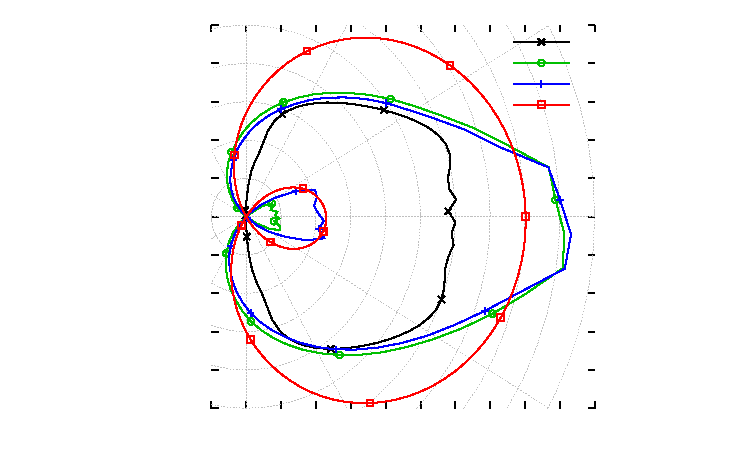
\includegraphics{/Users/seth/_thesis/figures/crashpipe2b/intens-x1-t1/intensity-x1-t1.pdf}}%
    \gplfronttext
  \end{picture}%
\endgroup

%  \hspace{-.5in}
%  \caption{Scalar flux with an isotropic boundary condition.}
%  \label{fig:isotropic}
%\end{figure}

\begin{figure}[tb]
  \centering
  \hspace{-.5in}
  % GNUPLOT: LaTeX picture with Postscript
\begingroup
  \makeatletter
  \providecommand\color[2][]{%
    \GenericError{(gnuplot) \space\space\space\@spaces}{%
      Package color not loaded in conjunction with
      terminal option `colourtext'%
    }{See the gnuplot documentation for explanation.%
    }{Either use 'blacktext' in gnuplot or load the package
      color.sty in LaTeX.}%
    \renewcommand\color[2][]{}%
  }%
  \providecommand\includegraphics[2][]{%
    \GenericError{(gnuplot) \space\space\space\@spaces}{%
      Package graphicx or graphics not loaded%
    }{See the gnuplot documentation for explanation.%
    }{The gnuplot epslatex terminal needs graphicx.sty or graphics.sty.}%
    \renewcommand\includegraphics[2][]{}%
  }%
  \providecommand\rotatebox[2]{#2}%
  \@ifundefined{ifGPcolor}{%
    \newif\ifGPcolor
    \GPcolortrue
  }{}%
  \@ifundefined{ifGPblacktext}{%
    \newif\ifGPblacktext
    \GPblacktexttrue
  }{}%
  % define a \g@addto@macro without @ in the name:
  \let\gplgaddtomacro\g@addto@macro
  % define empty templates for all commands taking text:
  \gdef\gplbacktext{}%
  \gdef\gplfronttext{}%
  \makeatother
  \ifGPblacktext
    % no textcolor at all
    \def\colorrgb#1{}%
    \def\colorgray#1{}%
  \else
    % gray or color?
    \ifGPcolor
      \def\colorrgb#1{\color[rgb]{#1}}%
      \def\colorgray#1{\color[gray]{#1}}%
      \expandafter\def\csname LTw\endcsname{\color{white}}%
      \expandafter\def\csname LTb\endcsname{\color{black}}%
      \expandafter\def\csname LTa\endcsname{\color{black}}%
      \expandafter\def\csname LT0\endcsname{\color[rgb]{1,0,0}}%
      \expandafter\def\csname LT1\endcsname{\color[rgb]{0,1,0}}%
      \expandafter\def\csname LT2\endcsname{\color[rgb]{0,0,1}}%
      \expandafter\def\csname LT3\endcsname{\color[rgb]{1,0,1}}%
      \expandafter\def\csname LT4\endcsname{\color[rgb]{0,1,1}}%
      \expandafter\def\csname LT5\endcsname{\color[rgb]{1,1,0}}%
      \expandafter\def\csname LT6\endcsname{\color[rgb]{0,0,0}}%
      \expandafter\def\csname LT7\endcsname{\color[rgb]{1,0.3,0}}%
      \expandafter\def\csname LT8\endcsname{\color[rgb]{0.5,0.5,0.5}}%
    \else
      % gray
      \def\colorrgb#1{\color{black}}%
      \def\colorgray#1{\color[gray]{#1}}%
      \expandafter\def\csname LTw\endcsname{\color{white}}%
      \expandafter\def\csname LTb\endcsname{\color{black}}%
      \expandafter\def\csname LTa\endcsname{\color{black}}%
      \expandafter\def\csname LT0\endcsname{\color{black}}%
      \expandafter\def\csname LT1\endcsname{\color{black}}%
      \expandafter\def\csname LT2\endcsname{\color{black}}%
      \expandafter\def\csname LT3\endcsname{\color{black}}%
      \expandafter\def\csname LT4\endcsname{\color{black}}%
      \expandafter\def\csname LT5\endcsname{\color{black}}%
      \expandafter\def\csname LT6\endcsname{\color{black}}%
      \expandafter\def\csname LT7\endcsname{\color{black}}%
      \expandafter\def\csname LT8\endcsname{\color{black}}%
    \fi
  \fi
  \setlength{\unitlength}{0.0500bp}%
  \begin{picture}(7200.00,4320.00)%
    \gplgaddtomacro\gplbacktext{%
      \csname LTb\endcsname%
      \put(1910,400){\makebox(0,0)[r]{\strut{} 0.1}}%
      \put(1910,768){\makebox(0,0)[r]{\strut{} 0.08}}%
      \put(1910,1136){\makebox(0,0)[r]{\strut{} 0.06}}%
      \put(1910,1504){\makebox(0,0)[r]{\strut{} 0.04}}%
      \put(1910,1872){\makebox(0,0)[r]{\strut{} 0.02}}%
      \put(1910,2240){\makebox(0,0)[r]{\strut{} 0}}%
      \put(1910,2607){\makebox(0,0)[r]{\strut{} 0.02}}%
      \put(1910,2975){\makebox(0,0)[r]{\strut{} 0.04}}%
      \put(1910,3343){\makebox(0,0)[r]{\strut{} 0.06}}%
      \put(1910,3711){\makebox(0,0)[r]{\strut{} 0.08}}%
      \put(1910,4079){\makebox(0,0)[r]{\strut{} 0.1}}%
      \csname LTb\endcsname%
      \put(2030,200){\makebox(0,0){\strut{} 0.02}}%
      \csname LTb\endcsname%
      \put(2364,200){\makebox(0,0){\strut{} 0}}%
      \csname LTb\endcsname%
      \put(2699,200){\makebox(0,0){\strut{} 0.02}}%
      \csname LTb\endcsname%
      \put(3033,200){\makebox(0,0){\strut{} 0.04}}%
      \csname LTb\endcsname%
      \put(3368,200){\makebox(0,0){\strut{} 0.06}}%
      \csname LTb\endcsname%
      \put(3702,200){\makebox(0,0){\strut{} 0.08}}%
      \csname LTb\endcsname%
      \put(4037,200){\makebox(0,0){\strut{} 0.1}}%
      \csname LTb\endcsname%
      \put(4371,200){\makebox(0,0){\strut{} 0.12}}%
      \csname LTb\endcsname%
      \put(4706,200){\makebox(0,0){\strut{} 0.14}}%
      \csname LTb\endcsname%
      \put(5040,200){\makebox(0,0){\strut{} 0.16}}%
      \csname LTb\endcsname%
      \put(5375,200){\makebox(0,0){\strut{} 0.18}}%
      \csname LTb\endcsname%
      \put(5709,200){\makebox(0,0){\strut{} 0.2}}%
      \csname LTb\endcsname%
      \put(1330,2239){\rotatebox{-270}{\makebox(0,0){\strut{}x1 center $(1.01,3.5)$}}}%
    }%
    \gplgaddtomacro\gplfronttext{%
      \csname LTb\endcsname%
      \put(4806,3916){\makebox(0,0)[r]{\strut{}S$_{128}$}}%
      \csname LTb\endcsname%
      \put(4806,3716){\makebox(0,0)[r]{\strut{}FLAD$_{64}$}}%
      \csname LTb\endcsname%
      \put(4806,3516){\makebox(0,0)[r]{\strut{}AD$_{64}$}}%
      \csname LTb\endcsname%
      \put(4806,3316){\makebox(0,0)[r]{\strut{}FLD}}%
    }%
    \gplbacktext
    \put(0,0){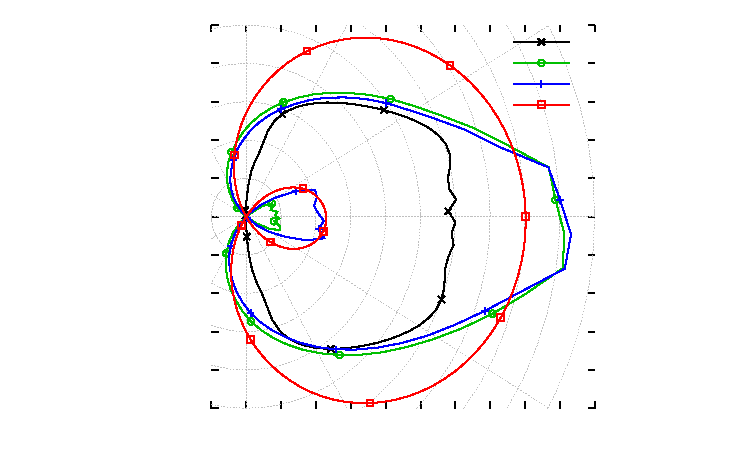
\includegraphics{/Users/seth/_thesis/figures/crashpipe2b/intens-x1-t1/intensity-x1-t1.pdf}}%
    \gplfronttext
  \end{picture}%
\endgroup

  \hspace{-.5in}
  \caption{Scalar flux with a normally incident boundary condition.}
  \label{fig:delta}
\end{figure}

%\begin{figure}[tbh!]
%  \centering
%  \hspace{-.5in}
%  % GNUPLOT: LaTeX picture with Postscript
\begingroup
  \makeatletter
  \providecommand\color[2][]{%
    \GenericError{(gnuplot) \space\space\space\@spaces}{%
      Package color not loaded in conjunction with
      terminal option `colourtext'%
    }{See the gnuplot documentation for explanation.%
    }{Either use 'blacktext' in gnuplot or load the package
      color.sty in LaTeX.}%
    \renewcommand\color[2][]{}%
  }%
  \providecommand\includegraphics[2][]{%
    \GenericError{(gnuplot) \space\space\space\@spaces}{%
      Package graphicx or graphics not loaded%
    }{See the gnuplot documentation for explanation.%
    }{The gnuplot epslatex terminal needs graphicx.sty or graphics.sty.}%
    \renewcommand\includegraphics[2][]{}%
  }%
  \providecommand\rotatebox[2]{#2}%
  \@ifundefined{ifGPcolor}{%
    \newif\ifGPcolor
    \GPcolortrue
  }{}%
  \@ifundefined{ifGPblacktext}{%
    \newif\ifGPblacktext
    \GPblacktexttrue
  }{}%
  % define a \g@addto@macro without @ in the name:
  \let\gplgaddtomacro\g@addto@macro
  % define empty templates for all commands taking text:
  \gdef\gplbacktext{}%
  \gdef\gplfronttext{}%
  \makeatother
  \ifGPblacktext
    % no textcolor at all
    \def\colorrgb#1{}%
    \def\colorgray#1{}%
  \else
    % gray or color?
    \ifGPcolor
      \def\colorrgb#1{\color[rgb]{#1}}%
      \def\colorgray#1{\color[gray]{#1}}%
      \expandafter\def\csname LTw\endcsname{\color{white}}%
      \expandafter\def\csname LTb\endcsname{\color{black}}%
      \expandafter\def\csname LTa\endcsname{\color{black}}%
      \expandafter\def\csname LT0\endcsname{\color[rgb]{1,0,0}}%
      \expandafter\def\csname LT1\endcsname{\color[rgb]{0,1,0}}%
      \expandafter\def\csname LT2\endcsname{\color[rgb]{0,0,1}}%
      \expandafter\def\csname LT3\endcsname{\color[rgb]{1,0,1}}%
      \expandafter\def\csname LT4\endcsname{\color[rgb]{0,1,1}}%
      \expandafter\def\csname LT5\endcsname{\color[rgb]{1,1,0}}%
      \expandafter\def\csname LT6\endcsname{\color[rgb]{0,0,0}}%
      \expandafter\def\csname LT7\endcsname{\color[rgb]{1,0.3,0}}%
      \expandafter\def\csname LT8\endcsname{\color[rgb]{0.5,0.5,0.5}}%
    \else
      % gray
      \def\colorrgb#1{\color{black}}%
      \def\colorgray#1{\color[gray]{#1}}%
      \expandafter\def\csname LTw\endcsname{\color{white}}%
      \expandafter\def\csname LTb\endcsname{\color{black}}%
      \expandafter\def\csname LTa\endcsname{\color{black}}%
      \expandafter\def\csname LT0\endcsname{\color{black}}%
      \expandafter\def\csname LT1\endcsname{\color{black}}%
      \expandafter\def\csname LT2\endcsname{\color{black}}%
      \expandafter\def\csname LT3\endcsname{\color{black}}%
      \expandafter\def\csname LT4\endcsname{\color{black}}%
      \expandafter\def\csname LT5\endcsname{\color{black}}%
      \expandafter\def\csname LT6\endcsname{\color{black}}%
      \expandafter\def\csname LT7\endcsname{\color{black}}%
      \expandafter\def\csname LT8\endcsname{\color{black}}%
    \fi
  \fi
  \setlength{\unitlength}{0.0500bp}%
  \begin{picture}(7200.00,4320.00)%
    \gplgaddtomacro\gplbacktext{%
      \csname LTb\endcsname%
      \put(1910,400){\makebox(0,0)[r]{\strut{} 0.1}}%
      \put(1910,768){\makebox(0,0)[r]{\strut{} 0.08}}%
      \put(1910,1136){\makebox(0,0)[r]{\strut{} 0.06}}%
      \put(1910,1504){\makebox(0,0)[r]{\strut{} 0.04}}%
      \put(1910,1872){\makebox(0,0)[r]{\strut{} 0.02}}%
      \put(1910,2240){\makebox(0,0)[r]{\strut{} 0}}%
      \put(1910,2607){\makebox(0,0)[r]{\strut{} 0.02}}%
      \put(1910,2975){\makebox(0,0)[r]{\strut{} 0.04}}%
      \put(1910,3343){\makebox(0,0)[r]{\strut{} 0.06}}%
      \put(1910,3711){\makebox(0,0)[r]{\strut{} 0.08}}%
      \put(1910,4079){\makebox(0,0)[r]{\strut{} 0.1}}%
      \csname LTb\endcsname%
      \put(2030,200){\makebox(0,0){\strut{} 0.02}}%
      \csname LTb\endcsname%
      \put(2364,200){\makebox(0,0){\strut{} 0}}%
      \csname LTb\endcsname%
      \put(2699,200){\makebox(0,0){\strut{} 0.02}}%
      \csname LTb\endcsname%
      \put(3033,200){\makebox(0,0){\strut{} 0.04}}%
      \csname LTb\endcsname%
      \put(3368,200){\makebox(0,0){\strut{} 0.06}}%
      \csname LTb\endcsname%
      \put(3702,200){\makebox(0,0){\strut{} 0.08}}%
      \csname LTb\endcsname%
      \put(4037,200){\makebox(0,0){\strut{} 0.1}}%
      \csname LTb\endcsname%
      \put(4371,200){\makebox(0,0){\strut{} 0.12}}%
      \csname LTb\endcsname%
      \put(4706,200){\makebox(0,0){\strut{} 0.14}}%
      \csname LTb\endcsname%
      \put(5040,200){\makebox(0,0){\strut{} 0.16}}%
      \csname LTb\endcsname%
      \put(5375,200){\makebox(0,0){\strut{} 0.18}}%
      \csname LTb\endcsname%
      \put(5709,200){\makebox(0,0){\strut{} 0.2}}%
      \csname LTb\endcsname%
      \put(1330,2239){\rotatebox{-270}{\makebox(0,0){\strut{}x1 center $(1.01,3.5)$}}}%
    }%
    \gplgaddtomacro\gplfronttext{%
      \csname LTb\endcsname%
      \put(4806,3916){\makebox(0,0)[r]{\strut{}S$_{128}$}}%
      \csname LTb\endcsname%
      \put(4806,3716){\makebox(0,0)[r]{\strut{}FLAD$_{64}$}}%
      \csname LTb\endcsname%
      \put(4806,3516){\makebox(0,0)[r]{\strut{}AD$_{64}$}}%
      \csname LTb\endcsname%
      \put(4806,3316){\makebox(0,0)[r]{\strut{}FLD}}%
    }%
    \gplbacktext
    \put(0,0){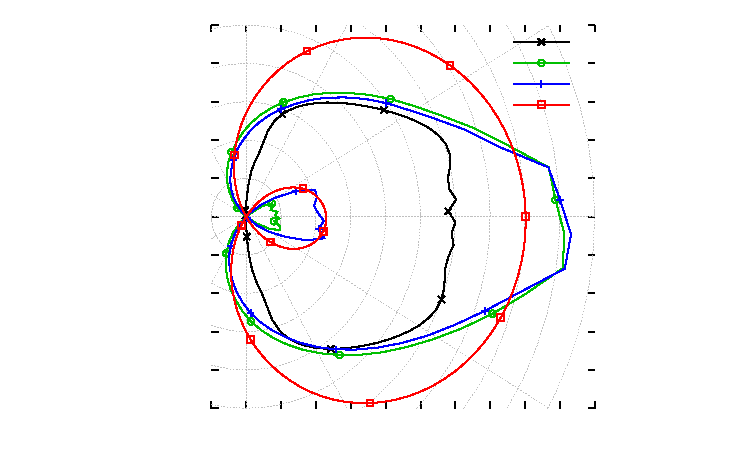
\includegraphics{/Users/seth/_thesis/figures/crashpipe2b/intens-x1-t1/intensity-x1-t1.pdf}}%
    \gplfronttext
  \end{picture}%
\endgroup

%  \hspace{-.5in}
%  \caption{Scalar flux with a grazing boundary condition.}
%  \label{fig:grazing}
%\end{figure}
%
\begin{figure}[tb]
  \centering
  \hspace{-.5in}
  % GNUPLOT: LaTeX picture with Postscript
\begingroup
  \makeatletter
  \providecommand\color[2][]{%
    \GenericError{(gnuplot) \space\space\space\@spaces}{%
      Package color not loaded in conjunction with
      terminal option `colourtext'%
    }{See the gnuplot documentation for explanation.%
    }{Either use 'blacktext' in gnuplot or load the package
      color.sty in LaTeX.}%
    \renewcommand\color[2][]{}%
  }%
  \providecommand\includegraphics[2][]{%
    \GenericError{(gnuplot) \space\space\space\@spaces}{%
      Package graphicx or graphics not loaded%
    }{See the gnuplot documentation for explanation.%
    }{The gnuplot epslatex terminal needs graphicx.sty or graphics.sty.}%
    \renewcommand\includegraphics[2][]{}%
  }%
  \providecommand\rotatebox[2]{#2}%
  \@ifundefined{ifGPcolor}{%
    \newif\ifGPcolor
    \GPcolortrue
  }{}%
  \@ifundefined{ifGPblacktext}{%
    \newif\ifGPblacktext
    \GPblacktexttrue
  }{}%
  % define a \g@addto@macro without @ in the name:
  \let\gplgaddtomacro\g@addto@macro
  % define empty templates for all commands taking text:
  \gdef\gplbacktext{}%
  \gdef\gplfronttext{}%
  \makeatother
  \ifGPblacktext
    % no textcolor at all
    \def\colorrgb#1{}%
    \def\colorgray#1{}%
  \else
    % gray or color?
    \ifGPcolor
      \def\colorrgb#1{\color[rgb]{#1}}%
      \def\colorgray#1{\color[gray]{#1}}%
      \expandafter\def\csname LTw\endcsname{\color{white}}%
      \expandafter\def\csname LTb\endcsname{\color{black}}%
      \expandafter\def\csname LTa\endcsname{\color{black}}%
      \expandafter\def\csname LT0\endcsname{\color[rgb]{1,0,0}}%
      \expandafter\def\csname LT1\endcsname{\color[rgb]{0,1,0}}%
      \expandafter\def\csname LT2\endcsname{\color[rgb]{0,0,1}}%
      \expandafter\def\csname LT3\endcsname{\color[rgb]{1,0,1}}%
      \expandafter\def\csname LT4\endcsname{\color[rgb]{0,1,1}}%
      \expandafter\def\csname LT5\endcsname{\color[rgb]{1,1,0}}%
      \expandafter\def\csname LT6\endcsname{\color[rgb]{0,0,0}}%
      \expandafter\def\csname LT7\endcsname{\color[rgb]{1,0.3,0}}%
      \expandafter\def\csname LT8\endcsname{\color[rgb]{0.5,0.5,0.5}}%
    \else
      % gray
      \def\colorrgb#1{\color{black}}%
      \def\colorgray#1{\color[gray]{#1}}%
      \expandafter\def\csname LTw\endcsname{\color{white}}%
      \expandafter\def\csname LTb\endcsname{\color{black}}%
      \expandafter\def\csname LTa\endcsname{\color{black}}%
      \expandafter\def\csname LT0\endcsname{\color{black}}%
      \expandafter\def\csname LT1\endcsname{\color{black}}%
      \expandafter\def\csname LT2\endcsname{\color{black}}%
      \expandafter\def\csname LT3\endcsname{\color{black}}%
      \expandafter\def\csname LT4\endcsname{\color{black}}%
      \expandafter\def\csname LT5\endcsname{\color{black}}%
      \expandafter\def\csname LT6\endcsname{\color{black}}%
      \expandafter\def\csname LT7\endcsname{\color{black}}%
      \expandafter\def\csname LT8\endcsname{\color{black}}%
    \fi
  \fi
  \setlength{\unitlength}{0.0500bp}%
  \begin{picture}(7200.00,4320.00)%
    \gplgaddtomacro\gplbacktext{%
      \csname LTb\endcsname%
      \put(1910,400){\makebox(0,0)[r]{\strut{} 0.1}}%
      \put(1910,768){\makebox(0,0)[r]{\strut{} 0.08}}%
      \put(1910,1136){\makebox(0,0)[r]{\strut{} 0.06}}%
      \put(1910,1504){\makebox(0,0)[r]{\strut{} 0.04}}%
      \put(1910,1872){\makebox(0,0)[r]{\strut{} 0.02}}%
      \put(1910,2240){\makebox(0,0)[r]{\strut{} 0}}%
      \put(1910,2607){\makebox(0,0)[r]{\strut{} 0.02}}%
      \put(1910,2975){\makebox(0,0)[r]{\strut{} 0.04}}%
      \put(1910,3343){\makebox(0,0)[r]{\strut{} 0.06}}%
      \put(1910,3711){\makebox(0,0)[r]{\strut{} 0.08}}%
      \put(1910,4079){\makebox(0,0)[r]{\strut{} 0.1}}%
      \csname LTb\endcsname%
      \put(2030,200){\makebox(0,0){\strut{} 0.02}}%
      \csname LTb\endcsname%
      \put(2364,200){\makebox(0,0){\strut{} 0}}%
      \csname LTb\endcsname%
      \put(2699,200){\makebox(0,0){\strut{} 0.02}}%
      \csname LTb\endcsname%
      \put(3033,200){\makebox(0,0){\strut{} 0.04}}%
      \csname LTb\endcsname%
      \put(3368,200){\makebox(0,0){\strut{} 0.06}}%
      \csname LTb\endcsname%
      \put(3702,200){\makebox(0,0){\strut{} 0.08}}%
      \csname LTb\endcsname%
      \put(4037,200){\makebox(0,0){\strut{} 0.1}}%
      \csname LTb\endcsname%
      \put(4371,200){\makebox(0,0){\strut{} 0.12}}%
      \csname LTb\endcsname%
      \put(4706,200){\makebox(0,0){\strut{} 0.14}}%
      \csname LTb\endcsname%
      \put(5040,200){\makebox(0,0){\strut{} 0.16}}%
      \csname LTb\endcsname%
      \put(5375,200){\makebox(0,0){\strut{} 0.18}}%
      \csname LTb\endcsname%
      \put(5709,200){\makebox(0,0){\strut{} 0.2}}%
      \csname LTb\endcsname%
      \put(1330,2239){\rotatebox{-270}{\makebox(0,0){\strut{}x1 center $(1.01,3.5)$}}}%
    }%
    \gplgaddtomacro\gplfronttext{%
      \csname LTb\endcsname%
      \put(4806,3916){\makebox(0,0)[r]{\strut{}S$_{128}$}}%
      \csname LTb\endcsname%
      \put(4806,3716){\makebox(0,0)[r]{\strut{}FLAD$_{64}$}}%
      \csname LTb\endcsname%
      \put(4806,3516){\makebox(0,0)[r]{\strut{}AD$_{64}$}}%
      \csname LTb\endcsname%
      \put(4806,3316){\makebox(0,0)[r]{\strut{}FLD}}%
    }%
    \gplbacktext
    \put(0,0){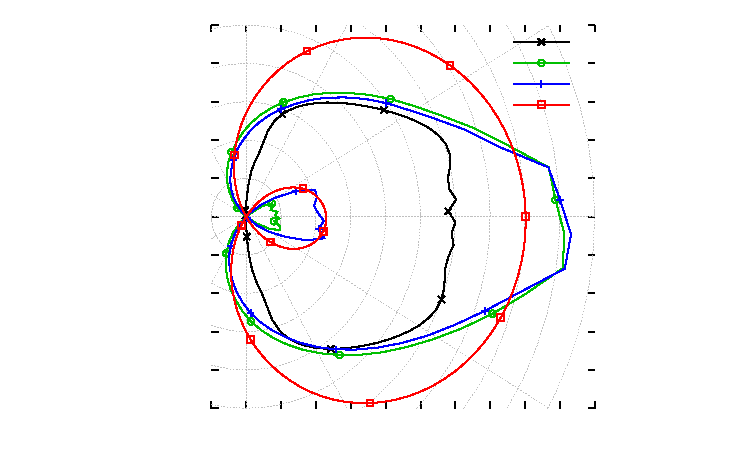
\includegraphics{/Users/seth/_thesis/figures/crashpipe2b/intens-x1-t1/intensity-x1-t1.pdf}}%
    \gplfronttext
  \end{picture}%
\endgroup

  \hspace{-.5in}
  \caption{Relative errors ($\phi/\phi_\text{MC} - 1$) of the three tested
  distributions.}
  \label{fig:relative}
\end{figure}

%%%%%%%%%%%%%%%%%%%%%%%%%%%%%%%%%%%%%%%%%%%%%%%%%%%%%%%%%%%%%%%%%%%%%%%%%%%%%%%%
\section{Conclusions}
We have derived and tested Marshak and variational boundary
conditions for the diffusion approximation to the transport equation in
flatland geometry. 

The Marshak boundary condition, which uses $\pi \int_{\vec{\Omega}\vd \vec{n} <
0 } \abs{\vec{\Omega}\vd \vec{n}} \psi^b \ud\Omega$, gives an extrapolation
distance of about $0.7854$.  The variational boundary condition given in
Eq.~\eqref{eq:flatVarBc} uses $\int_{\vec{\Omega}\vd\vec{n} < 0} \left[
\frac{\pi}{2} \abs{\vec{\Omega}\vd\vec{n}} + 2 (\vec{\Omega}\vd\vec{n})^2
\right] \psi^b(\vec{x}, \vec{\Omega}) \ud\Omega$ with the extrapolation
distance of about $0.8171$. Numerical simulations show that the variational
boundary condition is significantly more accurate than the Marshak condition,
especially for anisotropic incident boundary fluxes $\psi^b$. Overall, the
flatland Marshak and variational diffusion boundary conditions have accuracies
comparable to their 3-D counterparts. 

These results have application in the testing of numerical methods for multi-D
transport problems. The flatland implementation of these methods is easier and
less costly than in standard 2-D or 3-D geometries, and the results seen in
flatland are strongly correlated to results in 2-D and 3-D.

%%%%%%%%%%%%%%%%%%%%%%%%%%%%%%%%%%%%%%%%%%%%%%%%%%%%%%%%%%%%%%%%%%%%%%%%%%%%%%%%
\section{Acknowledgments}
This material is based upon work supported under a Department of Energy Nuclear
Energy University Programs Graduate Fellowship.

%%%%%%%%%%%%%%%%%%%%%%%%%%%%%%%%%%%%%%%%%%%%%%%%%%%%%%%%%%%%%%%%%%%%%%%%%%%%%%%%
\bibliographystyle{ans}
\bibliography{../SRJall}
\end{document}

